% Chapter 1

\chapter{Introduction} % Main chapter title

\label{Chapter1} % For referencing the chapter elsewhere, use \ref{Chapter1}

% L'introduction situe le problème, l'expose, insiste sur son importance et indique la manière dont il est envisagé. A l'introduction est associée une  présentation préliminaire de la manière de traiter la question (méthode). L'introduction doit aussi exposer l’étude de l’existant dans le domaine précis qui concerne le PFE et faire ressortir la nécessité de réalisations complémentaires comme celle qui fait l'objet du PFE.

\section{Motivation}

\paragraph{} Service robotics are an active research field: there is a growing demand for intelligent machines that are meant to be used in human environments for domestic tasks (e.g, maintaining people homes, entertaining them, caring for them; especially old ones or with disabilities, \dots) \cmmnt{\parencite{mettler_service_2017, graf_care-o-bot_2004}}. To fulfill such tasks, a service robot obviously needs to be able to autonomously navigate through space, according to the given constraints: these navigation capabilities and constraints are the main focus of the following work.

\paragraph{} Human environments represent a very complex challenge, since they are dynamic, alterable and imply social conventions and rules that the robot must also respect in the way it navigates and interacts with the world. For example, in a home, humans (or other autonomous actors, such as pets) are moving obstacles that must be taken into account. Also, for a robot to go from a point A to B, a solution may only be found if it implies moving an obstacle out of the way. And all this must be done in socially acceptable manner: one would not appreciate a robot moving at high speeds around people or to move obstacles that are not supposed to be moved.

\paragraph{} The most common constraint for robot navigation is solely to find the shortest collision-free path, and this is an acceptable solution in a static context (nothing moves, at the exception of the robot). However, if we want the robot to navigate a human environment as described above, this is not sufficient.

\begin{figure}[H]
\centering
\begin{subfigure}{.5\textwidth}
  \centering
  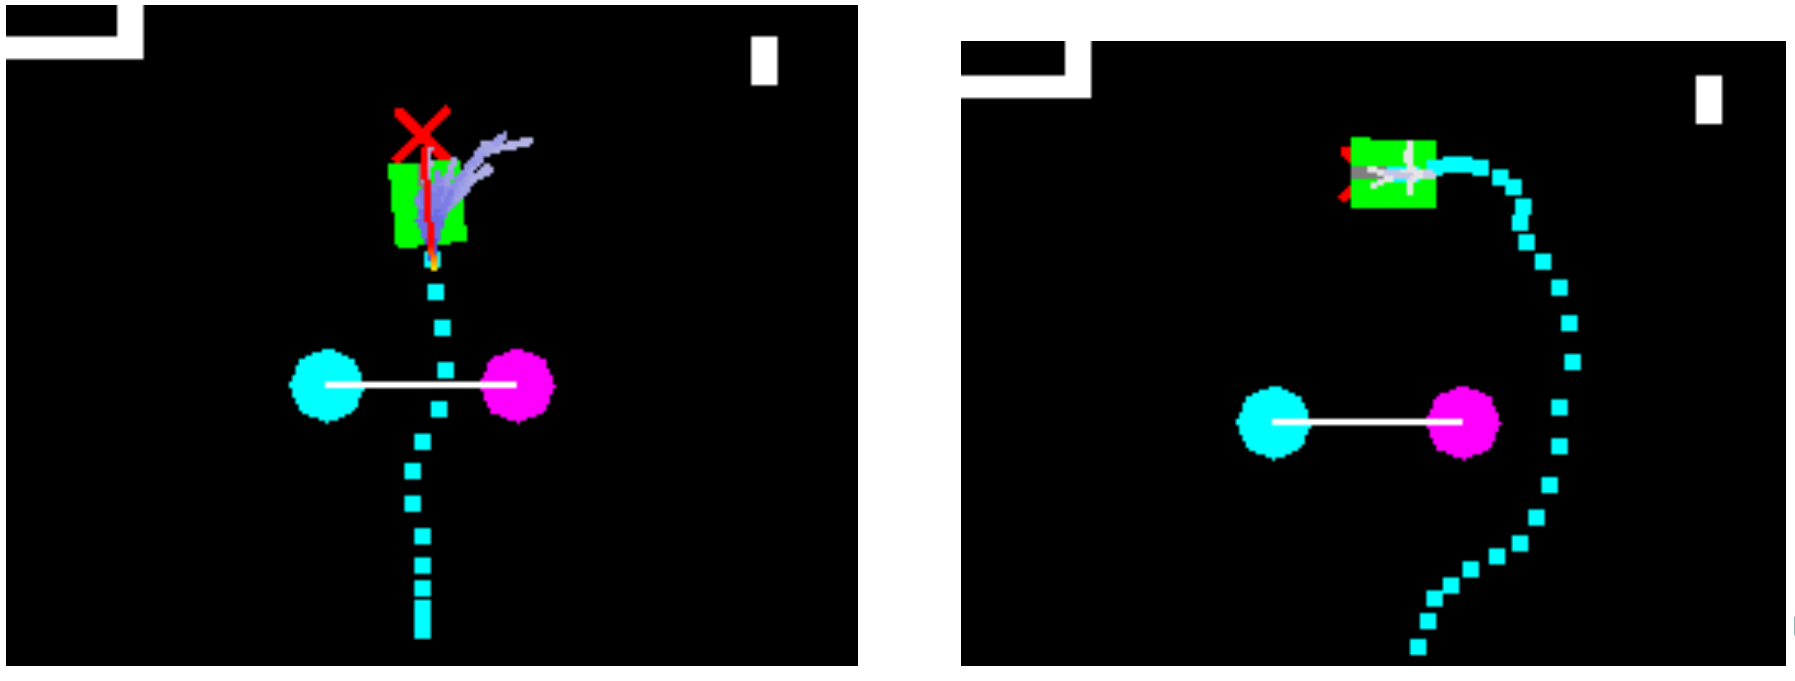
\includegraphics[width=0.9\linewidth]{Figures/Problem_Illustration/social_problem.png}
  \caption{Sample social navigation problem}
  \label{fig:social_problem}
\end{subfigure}%
\begin{subfigure}{.5\textwidth}
  \centering
  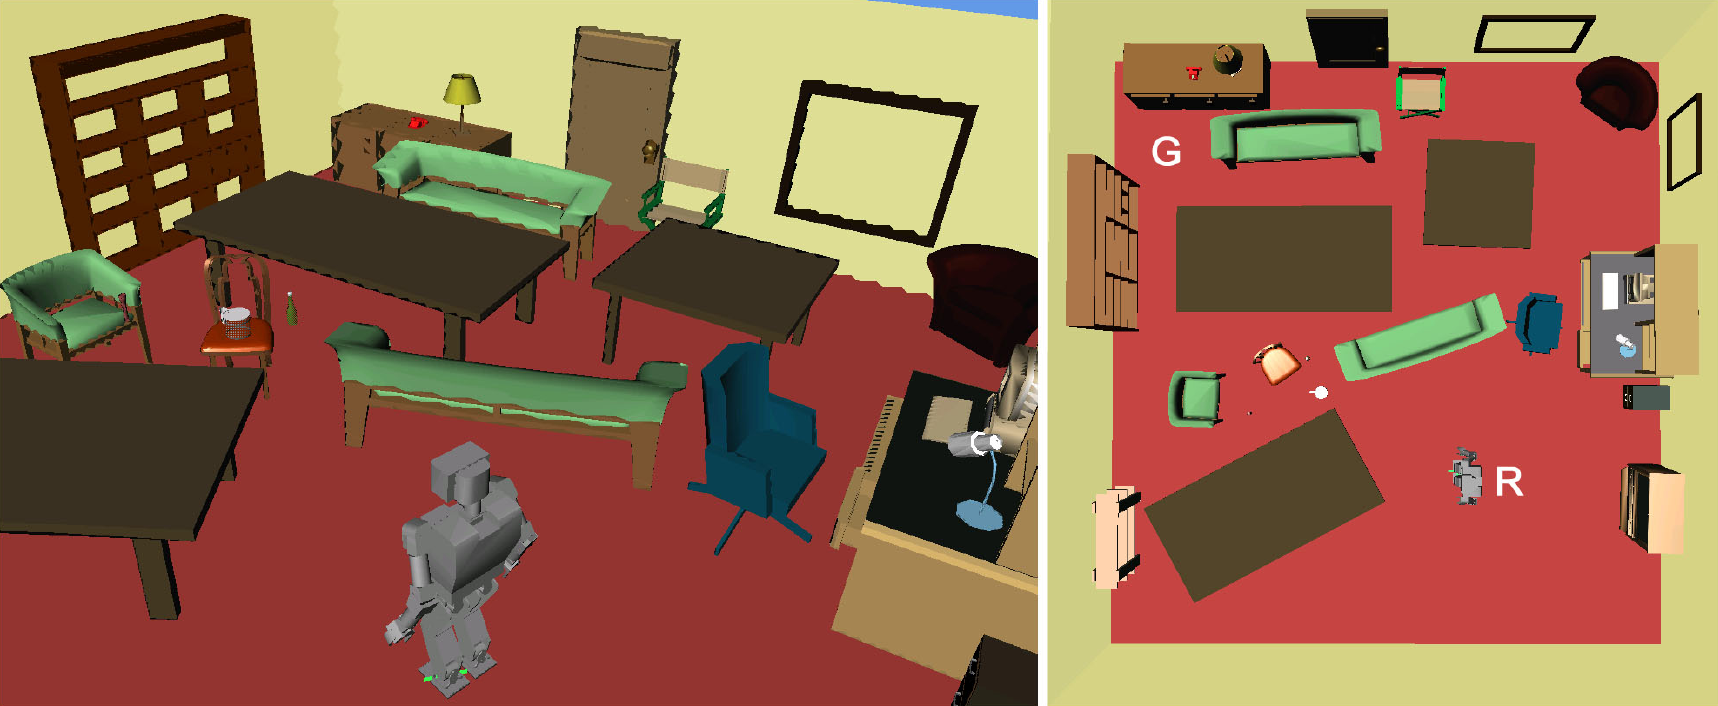
\includegraphics[width=0.9\linewidth]{Figures/Problem_Illustration/namo_problem.png}
  \caption{Sample NAMO problem}
  \label{fig:namo_problem}
\end{subfigure}
\caption{Sample problems for social navigation and NAMO. In the sample social navigation problem, the robot (green square) must reconsider its path to avoid penetrating the zone between the two humans (colored dots) interacting with each other (image from \parencite{rios-martinez_understanding_2011}). In the NAMO problem,  the robot will need to move obstacles in order to access its goal (image from \parencite{stilman_navigation_2005}).}
\label{fig:navigation_problems}
\end{figure}

\paragraph{} To our knowledge, the problem of navigation planning in dynamic environments populated with humans \parencite{kruse_human-aware_2013, rios-martinez_proxemics_2015}, and the problem of navigation planning in robot-alterable environments (which is called Navigation Among Movable Obstacles, or NAMO, more precisely defined in \parencite{stilman_navigation_2007}) have always been treated separately. The \groupname \footnote{Team website: \url{https://team.inria.fr/chroma/}} \, for one, proposed social and dynamic navigation algorithms that optimize the generation of trajectories by managing the risk of colliding with obstacles \parencite{fulgenzi_autonomous_2009, rios-martinez_socially-aware_2013}, respecting social conventions such as avoiding human interaction spaces \parencite{papadakis_adaptive_2014, rios-martinez_understanding_2011} (Figure \ref{fig:social_problem}), or predicting the trajectories of moving obstacles \parencite{jumel_mapping_2017}, \dots The NAMO problem (Figure \ref{fig:namo_problem}) has been dealt with in a great variety of contexts, detailed in Chapter \ref{Chapter2}. It seems that these two problems have yet to be brought together, and the new problematics that are to arise from this confluence are still to be identified and addressed.

\section{Objective}

\paragraph{} The long-term objective behind this work is to allow a service robot to navigate in complex, human, dynamic and robot-alterable environments, preferably in an optimal way (minimize risk of collision, travel distance, time or energy, \dots).

\paragraph{} More precisely, the context of this long-term objective for formulating, comparing and evaluating hypotheses, is the Robocup@Home\footnote{Competition website: \url{http://www.robocupathome.org/}}. The \groupname \, participates in the standard league of this international-level competition, that provides service robotics challenges to evaluate solutions proposed by researchers and students. The mandatory robotic platform for the standard league is the Pepper robot \footnote{Pepper characteristics: \url{http://doc.aldebaran.com/2-4/family/pepper_technical/index_dev_pepper.html}}, piloted through ROS \footnote{ROS, the Robot Operating System, website: \url{http://www.ros.org/}} for our team. Notably, this defines the context of our search in that:
\begin{itemize}
  \item only the onboard sensors of the robot are used to update the robot's \textbf{partial environment knowledge} making,
  \item we thus seek \textbf{local optimality}: that is, optimal decision-making given the current belief state of the robot on its environment,
  \item overall, we will privilegiate solutions that are more easily applicable for Pepper. For example, we will prefer a solution that involves pushing rather than grasping obstacles to move them, as Pepper's limited mechanical features make it difficult to grasp obstacles in a safe way for the robot.
\end{itemize}

\paragraph{} In the end, the specific objectives of this first work are to:
\begin{itemize}
  \item explore the NAMO problem domain and extract characteristics that allow to sort through existing works,
  \item identify both new concerns and bridges between this problem and the ones of dynamic and social navigation,
  \item and finally build upon existing work to propose solutions to the previously identified concerns.
\end{itemize}

\clearpage

\section{Overview}

\paragraph{} The following work is organized as follows:

\begin{itemize}
  \item Chapter \ref{Chapter2} is a detailed state of the art of the NAMO domain, and derives comparison criteria from a selection of articles that are closely related to our goals. It also explains the choice of the papers we chose to build upon.
  \item Chapter \ref{Chapter3} is a thorough study and criticism of the chosen base algorithm. We explain the logic of the original algorithm while also providing definitions and conventions that remove the many original ambiguities. Finally, we propose a pseudocode interpretation of the improvements proposed by Levihn et. al. on the first algorithm.
  \item Chapter \ref{Chapter4} revisits the algorithm to really restore optimality, make it stick to our hypotheses, and extend it to solve new social and dynamic environment concerns.
  \item Chapter \ref{Chapter5} recounts our experimentations with the Pepper robot and simulations to validate our propositions.
  \item Chapter \ref{Chapter6} summarizes our contributions and details opportunities for research arisen by this work.
  \item Appendices \ref{algorithms} and \ref{comparison_tables} gather comparison tables and pseudocode representations of algorithm propositions.
\end{itemize}
